\documentclass{standalone}

\usepackage{tikz,pgfplots}

\pgfplotsset{compat=1.18}
\pgfplotsset{
	soldot/.style={
		color=black,only marks,mark=*},
	holdot/.style={
		color=black,fill=white,only marks,mark=*},
	compat=1.12,
	standard/.style={
     		every axis x label/.style={at={(current axis.right of origin)},anchor=north west},
    		every axis y label/.style={at={(current axis.above origin)},anchor=north east}}
}

\usetikzlibrary{calc}
\usetikzlibrary{intersections}
\usetikzlibrary{decorations.markings}
\usetikzlibrary{arrows.meta}
\tikzset{>={Latex[scale=1.2]}}

\begin{document}

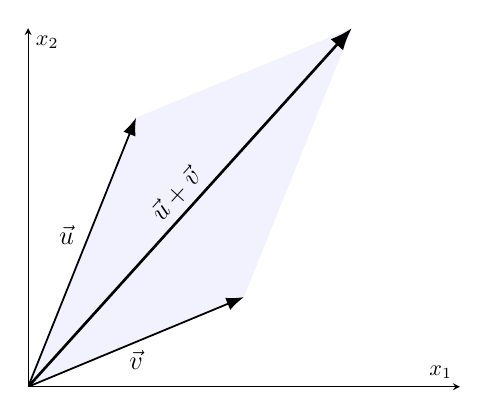
\begin{tikzpicture}[scale=0.8]
\begin{axis}[grid=none,
axis lines=middle,
xmin=0,xmax=4,
ymin=0,ymax=4,
xtick=\empty,
ytick=\empty,
minor tick={},
xlabel=\(x_1\), ylabel=\(x_2\),
samples=250]
\fill[blue!5] (0,0) -- (1,3) -- (3,4) -- (2,1) --cycle;
\draw[->,thick] (0,0) -- (1,3) node[midway,above left] {\large$\vec{u}$};
\draw[->,thick] (0,0) -- (2,1) node[midway, below] {\large$\vec{v}$};
\draw[->,very thick] (0,0) -- (3,4) node[midway,above,sloped] {\large$\vec{u} + \vec{v}$};
\end{axis}
\end{tikzpicture}

\end{document}